\chapter{Introduction}
\label{ch1}

%%%%%%%%%%%%%%%%%%%%%%%%%%%%%%%%%%%%%%%
% IMPORTANT
\begin{spacing}{1.25} %THESE FOUR
\minitoc % LINES MUST APPEAR IN
\end{spacing} % EVERY
\onehalfspacing % CHAPTER
% COPY THEM IN ANY NEW CHAPTER
%%%%%%%%%%%%%%%%%%%%%%%%%%%%%%%%%%%%%%%

\section{Background}

Since the 18th century, iron, steel, and concrete have replaced timber and stone in the design, manufacture, and construction of large modern structures, including bridges. In the case of steel structures, components are factory-manufactured and then delivered to the construction site, where they are assembled or connected on site. Units are transported in members that are manufactured in factories. The members consist mostly of steel plates, and the main objective is to connect them together through a process called 'splicing'.

Steel bridges constructed between 1860 and 1955 were predominantly connected with riveted joints \cite{Quentin2012MorphogenesisStructures, COLLETTE2014, Ambroziak2023CASEANALYSIS, Collette2012Les18401940, Costa2013RehabilitationBridge}, as shown in Fig.\ref{fig-intro1} (Photo by Luca Upper \cite{lucaphoto}). In Japan, the period of cast iron started in 1897 which later shifted towards steel industry. The joints were riveted until the introduction of welding in the 1950s, where 40 kg grade SS39A and SS41 structural steel were used \cite{rivet1934}. This ancient type of joint allows secure connection of two or more metal sheets. Rivets are placed in the hole, then heated to high temperature by a pneumatic hammer which forms a head. After it cools down, a residual clamping force is created, making a riveted joint possible.

\begin{figure}[htbp]
    \centering
    
\includegraphics[width=0.85\textwidth]{imgs/intro/steel-structure.jpg}
    \caption{Riveted joint of railway bridge in Switzerland (Photo by Luca Upper)}
    \label{fig-intro1}
\end{figure}

After 1955, advancements in steel technology enabled the production of high-strength steel. As a result of the bolt's ease of construction and its reliable mechanical transmission mechanism, it quickly supplanted the rivet as the prevailing joining method.

\ac{HSB} have three types of connection: friction connection, bearing connection, and tension connection. Out of these, the friction connection is the most commonly used.

\ac{Friction type connections} (also referred to as friction connections) involve joining materials that transmit stress through frictional resistance generated by the inter-material compressive force produced when the jointing materials are tightened using high-strength bolts. Stress is transferred via compressive forces between materials that are dispersed around the bolt, unlike in riveted joints where stress is transmitted through local bearing forces. This results in decreased stress concentration and smoother flow of stress. Another advantage is there is no misalignment between the joined materials until the application of a force which exceeds the frictional resistance can cause the friction to break and slip to occur, thus ensuring exceptionally high rigidity and fatigue strength.

Welding was first applied to steel bridges in the 1930s \cite{ALENCAR2019154}. And arc welding was first invented in the late 19th century, with high-density energies, like electron and laser beams, being applied to welding in the late 20th century. Welding conncetions are usually carried out in the factory due to the stringent construction conditions on site.

%todo!

%Insert 3 type of joint
Each of the three different types of connection has its own advantages and disadvantages, and no combination can completely replace any of them. And occasionally it is necessary to use two different types of joint at the same time, probably because of the lack of skilled labour (for repair riveted bridge, rivet combined with \ac{HSB}), the inability of the joint surface to meet the required slip coefficients (Friction type combined with Bearing type connection) as well as the need to increase the strength of the joint to shorten the joint length (\ac{HSB} combined with welded connection), etc.

%hybrid history


\begin{figure}[htbp]
    \centering
    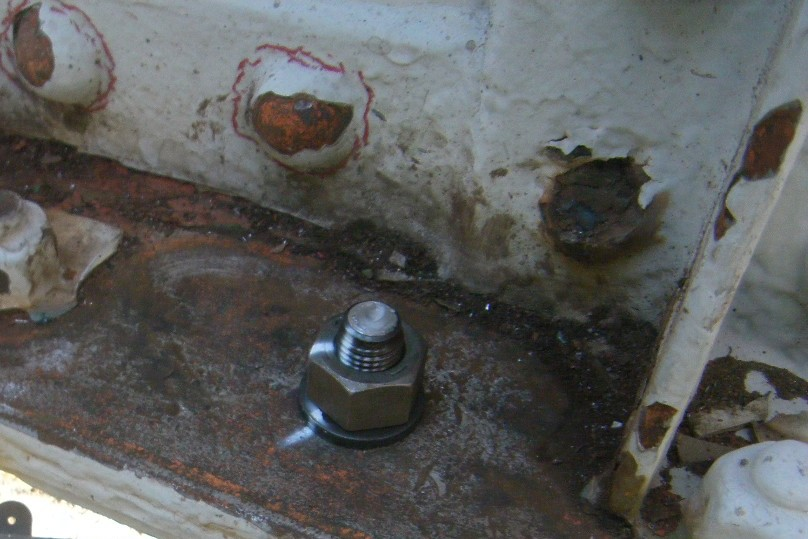
\includegraphics[width=0.8\textwidth]{imgs/intro/HSB-rivet.JPG}
    \caption{Rivet partially replaced by HSB of Hazukawa Riveted bridge in Fukui Japan}
    \label{fig-tprivet}
\end{figure}


\section{Technical Problem}

During the reconstruction projects following the Second World War, the combined use of diverse connection methods with varying principles presented challenges. For instance, when reinforcing aging riveted structures by welding or partially replacing them with \ac{HSB}, difficulties arose as shown in Fig. \ref{fig-tprivet}. Joining components with combined different load transfer mechanism connection methods results in a non-stationary structure, making it difficult to accurately calculate the sharing of loads in the past. As a result, only one of the two types was considered valid for design purposes at the time, ignoring the cooperative actions expected from their combined use.

The maintenance and repair of ageing bridges are expected to encounter growing obstacles in the near future. Bridges must achieve a compromise between suitable flexibility and rigidity. The addition of reinforcing elements to a completed bridge may upset this equilibrium and create problems. Consequently, post-construction reinforcement of a bridge may present a challenge by using \ac{FBHC}.

In addition, for new structural components, the rational use of \ac{FBHC} can effectively improve the strength of the joints and shorten the length of the joints as much as possible, while meeting the required strength to make the joint compact.  However, unlike the reinforcement of an existing structural component, new structural components raise issues of structural stability, durability and strict requirements for allowable deformation, and require a series of tests before they can be installed.

% In summary, this work focuses on the following technical issues for \ac{FBHC}:

% \begin{itemize}
%     \item The primary technical challenge lies in the lack of understanding regarding the load transfer mechanism of \ac{Hybrid connections}.
%     \item For the use of hybrid joints, not only to understand how the load is transmitted, but also to understand how the \ac{Fasteners} should be reasonably arranged. Different arrangements may produce different load transfer effects, so exploring the reasonable fastener arrangement scheme will be an important technical problem.
%     \item The stiffness of Friction connection and bearing connection are different. In the case of a friction connection, there will be a small elastic dislocation (slip) before occurrence, which is a different mechanical mechanism from the elastic deformation of a bearing connection. Exploring the deformation capacity of the bearing and friction combination is also an important technical subject.
%     \item After understanding the load transfer mechanism, strength and deformation performance of hybrid connections, it is necessary to define their limit states and to devise how to differentiate between the limit states and their corresponding strength equations.
    
% \end{itemize}


\section{Aims and Scope}

\subsection{Overall}

This work focused on the friction and bearing type hybrid connection (\ac{FBHC}). The thesis will be divided into two main parts for discussion. The first part entails repairing and enhancing aging riveted bridge through the replacement of damaged rivets with high-strength bolts using a friction connection. This technique is deployed to create hybrid joints that can jointly resist loads. The second part discusses the use of hybrid joints in the construction of new bridges. Such bridges encounter various design challenges, including the need to enhance component strength in response to increased external live loads without enlarging the structure size. These adjustments have become necessary in recent years, coinciding with the emergence and use of high-strength steels. The joints should be designed to withstand the increased strength of the steel components. However, the strength of friction joints is dependent on the number of bolts and slip coefficient. Enhancing the slip coefficient can effectively increase the joint strength, but this is an uncontrollable factor with significant construction costs. Therefore, it is imperative to suggest a cost-effective means of enhancing joint strength in high-strength steel structures without enlarging the joint size.


\subsection{Part 1: For Rivet-HSB hybrid connections}

For aging riveted bridges, the partial replacement of rivets with high-strength bolts creates \ac{FBHC}. This replacement process requires careful consideration of two aspects: the existing riveted connection's condition and the hybrid connection's mechanical behavior. The slip coefficient of aged riveted surfaces significantly influences the friction resistance, while the load redistribution during rivet replacement affects the joint's integrity. Furthermore, the distinct deformation characteristics between rivets and high-strength bolts necessitate a thorough understanding of their interaction in hybrid connections.

% This study addresses these challenges through the following objectives:

% \begin{enumerate}
%     \item Evaluate slip resistance of aged riveted surfaces
%     \item Analyze load redistribution mechanism during rivet replacement
%     \item Investigate load transfer behavior in hybrid connections
%     \item Establish strength calculation method for design
% \end{enumerate}


\subsection{Part 2: For IFB-HSB hybrid connections}

For newly constructed steel bridges, the combination of interference-fit bolts (\ac{IFB}) and high-strength bolts creates an innovative hybrid connection system. Unlike traditional fasteners, \ac{IFB}s serve as bearing-type connections while maintaining compatibility with \ac{HSB} friction connections. The mechanical behavior of this hybrid system presents unique characteristics, particularly regarding the effects of preload on \ac{IFB} bearing resistance and the interaction between different load transfer mechanisms.

% This study focuses on the following objectives:

% \begin{enumerate}
%     \item Evaluate the feasibility of \ac{IFB}-\ac{HSB} hybrid connections
%     \item Investigate preload effects on \ac{IFB} bearing performance
%     \item Analyze load transfer mechanisms and optimize bolt arrangements
%     \item Develop strength calculation methods for design applications
% \end{enumerate}

\subsection{Serviceability Limit State and Design Method for Hybrid Connections}

This study investigates the serviceability limit state and develops design methods for hybrid connections, including both Rivet-HSB and IFB-HSB combinations. Through numerical analysis and experimental validation, the research reveals three key aspects:

\begin{enumerate}
    \item Mechanical behavior: The hybrid connection exhibits distinct load transfer stages, from friction-dominant to bearing-dominant phases, with a transition stage in between.
    
    \item Load-sharing mechanism: The study quantifies the reduction in friction and bearing forces, proposing specific reduction factors ($\alpha_s$ and $\alpha_b$) for practical design.
    
    \item Design methodology: A comprehensive design approach is developed, accounting for the interaction between friction and bearing mechanisms while maintaining simplicity for practical applications.
\end{enumerate}

The findings provide a foundation for the reliable design of hybrid connections in steel structures, with validated strength calculation methods applicable to both Rivet-HSB and IFB-HSB configurations.

%todo-和overview的流程图一致,目的


\section{Research Approach And Thesis Outline}

This research follows a systematic approach as illustrated in Fig. \ref{fig-rflow}. Beginning with a literature review on bearing-type and friction-type connections, the study progresses through theoretical analysis, numerical simulation using \ac{FEA}, and experimental validation. The investigation focuses on both Rivet-\ac{HSB} and \ac{IFB}-\ac{HSB} hybrid connections, with the ultimate goal of clarifying their mechanical behavior, defining limit states, and developing practical design methods.


%research flow
\begin{figure}[htbp]
    \centering
    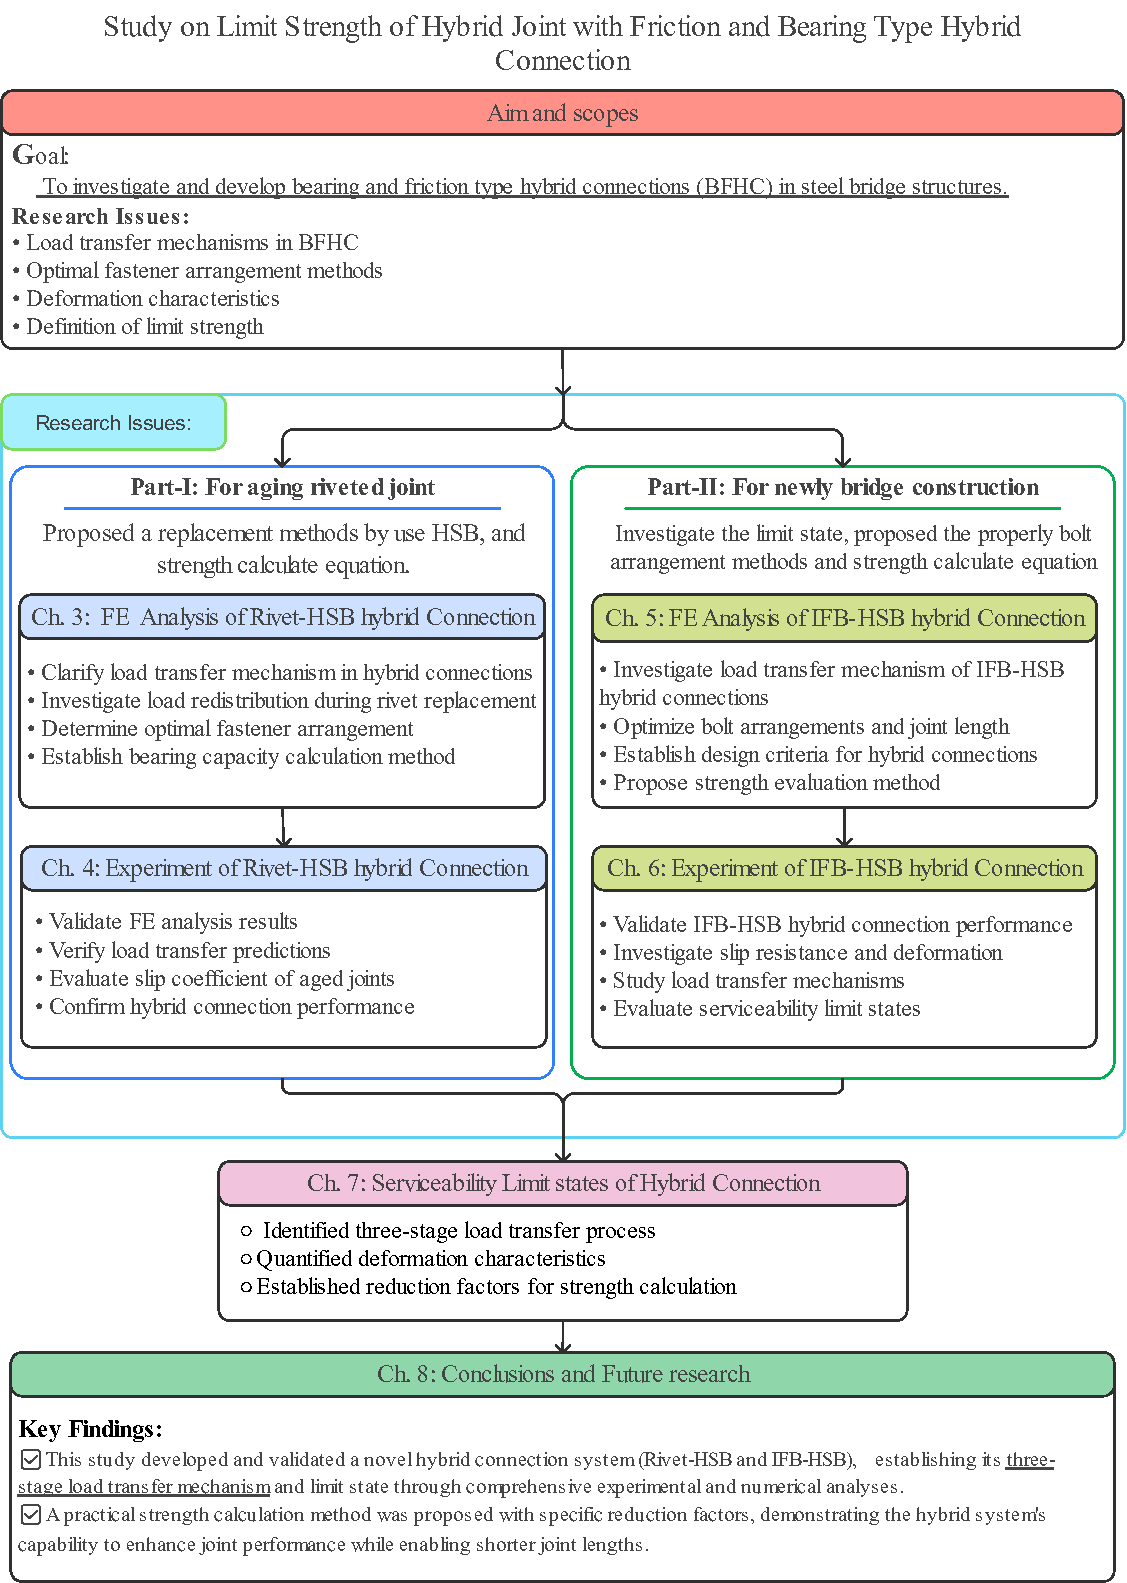
\includegraphics[width=\textwidth]{imgs/intro/research-flow.pdf}
    \caption{Overview of research flow}
    \label{fig-rflow}
\end{figure}